
\de{ĐỀ THI GIỮA HỌC KỲ II NĂM HỌC 2022-2023}{Phổ Thông Năng Khiếu}



\begin{bt}%[0D4K2-1]%[Dự án đề kiểm tra HKII NH22-23- Hiếu Mai]%[Phổ Thông Năng Khiếu]
Giải các phương trình, bất phương trình sau
	\begin{enumerate}
		\item $\dfrac{2x}{x^2-5x+6}\leq 1$
		\item $\sqrt{2x^2-3x+1}-\sqrt{x+1}=0$
		\item $\left(x^2+1\right)^2+3x\sqrt{x^2+2}-5=0$
	\end{enumerate}
\loigiai{
	\begin{enumerate}
	\item $\dfrac{2x}{x^2-5x+6}\leq 1$\\
Điều kiện: $x^2-5x+6\ne0 \Leftrightarrow \heva{&x\ne 2\\&x\ne 3.}$	\\
$\dfrac{2x}{x^2-5x+6}\leq 1 \Leftrightarrow \dfrac{-x^2+7x-6}{x^2-5x+6}\le0 $\\
Ta có bảng xét dấu
\begin{center}
\begin{tikzpicture}
	\tkzTabInit[nocadre=false,lgt=2,espcl=2,deltacl=0.5]
	{$x$/1 , $f(x)$/1 }
	{$-\infty$,$1$,$2$,$3$,$6$,$+\infty$}
	\tkzTabLine{,-,$0$,+,d,-,d,+,$0$,-}

\end{tikzpicture}
\end{center}
Vậy tập nghiệm của bất phương trình là $S=(-\infty;1] \cup (2;3) \cup [6;+\infty)$.
	\item $\sqrt{2x^2-3x+1}-\sqrt{x+1}=0$\\
	Điều kiện: $\heva{&2x^2-3x+1 \ge 0\\&x+1 \ge 0} \Leftrightarrow \heva{&-1 \le x \le \dfrac{1}{2}\\&x \ge 1.}$\\
$\sqrt{2x^2-3x+1}-\sqrt{x+1}=0 \\ \Leftrightarrow \sqrt{2x^2-3x+1}=\sqrt{ x+1}\\ \Leftrightarrow 2x^2-3x+1=x+1 \\ \Leftrightarrow 2x^2-4x=0 \Leftrightarrow \hoac{&x=0~ \text{(thỏa mãn)}\\&x=2~\text{(thỏa mãn)}.}$	
	\item $\left(x^2+1\right)^2+3x\sqrt{x^2+2}-5=0 \Leftrightarrow x^4+2x^2+1+3\sqrt{x^4+2x^2}-5=0 ~ (1)$.\\
	Đặt $\sqrt{x^4+2x^2}=t~ (t\ge 0)$.\\
	Phương trình $(1) \Leftrightarrow t^2+1+3t-5=0 \Leftrightarrow \hoac{&t=1\\&t=-4~\text{(loại).}}$\\
	Với $t=1\Leftrightarrow \sqrt{x^4+2x^2}=1 \Leftrightarrow x^4+2x^2=1 \Leftrightarrow \hoac{&x^2=-1+\sqrt{2}\\&x=-1-\sqrt{2}~\text{(loại)}}\\ \Leftrightarrow x=\pm \sqrt{-1+\sqrt{2}}$.
\end{enumerate}

}
\end{bt}

\begin{bt}%[0D4G2-1]%[Dự án đề kiểm tra HKII NH22-23- Hiếu Mai]%[Phổ Thông Năng Khiếu]
Tìm $m$ để hàm số $f(x)=\sqrt{\dfrac{x^2+1}{(m+2)x^2+2(m+2)x+m+3}}+m x+1$ có tập xác định là $\mathbb{R}$.
\loigiai{
Điều kiện: $\dfrac{x^2+1}{(m+2)x^2+2(m+2)x+m+3}\ge0$.\\
Vì $x^2+1 >0 ~\forall x\in \mathbb{R} $ nên $\dfrac{x^2+1}{(m+2)x^2+2(m+2)x+m+3}\ge0 \\ \Leftrightarrow (m+2)x^2+2(m+2)x+m+3 >0$.\\
Vậy để hàm số có tập xác định là $\mathbb{R}$ thì $(m+2)x^2+2(m+2)x+m+3 >0~\forall x\in \mathbb{R}$.\\
Trường hợp 1: Với $m=-2$ ta có $-2+3=1>0~\forall x\in \mathbb{R}$.\\
Trường hợp 2: Với $m\ne -2$ ta có $(m+2)x^2+2(m+2)x+m+3 >0~\forall x\in \mathbb{R}$\\
$\Leftrightarrow \heva{&m+2>0\\&\Delta'=(m+2)^2-(m+2)(m+3)<0 } \Leftrightarrow \heva{&m>-2\\&(m+2)(-1)<0} \Leftrightarrow m>-2$.\\
Vậy $m\ge -2$.
}
\end{bt}



\begin{bt}%[0T5K4-1]%[0T5K4-3]%[Dự án đề kiểm tra HKII NH22-23- Phan Trung Hiếu]%[Trường PTNK]
	Trong mặt phẳng $Oxy$, cho ba điểm $A(1;3)$, $B(3;1)$, $C(2;4)$.
	\begin{enumerate}
		\item Tính số đo góc $A$.
		\item Tìm điểm $M$ thuộc trục hoành sao cho tam giác $MAB$ vuông tại $M$. Tính diện tích tam giác $MAB$.
	\end{enumerate}
\loigiai{
\begin{enumerate}
\item Ta có
\begin{itemize}
	\item $\vv{AB} = (2;-2)$, suy ra $AB^2 = 2^2+(-2)^2 = 8$.
	\item  $\vv{AC} = (1;1)$, suy ra $AC^2 = 1^2+ 1^2=2$.
	\item $\vv{BC} = (-1;3)$, suy ra $BC^2 = (-1)^2+(3^2) = 10$.
\end{itemize}
Áp dụng hệ quả định lí Cosin trong tam giác $ABC$, ta có
\begin{equation*}
	\cos A = \dfrac{AB^2+AC^2-BC^2}{2\cdot AB\cdot AC} = \dfrac{8+2-10 }{2\cdot8\cdot2} = 0.
\end{equation*}
Suy ra, số đo góc $A$ là $\widehat{A}=90^\circ$.
\item Gọi tọa độ điểm $M$ thuộc trục hoành là $M(m,0)$.\\
Ta có
\begin{itemize}
	\item $\vv{AM} = (m-1;-3)$.
	\item $\vv{BM} = (m-3;-1)$.
\end{itemize} 
Để tam giác $MAB$ vuông tại $M$ thì
\begin{equation*}
	\vv{AM}\cdot\vv{BM}=0\Leftrightarrow (m-1)(m-3)+3 = 0 \Leftrightarrow m^2-4m +6 = 0\,(\text{Vô nghiệm}).
\end{equation*}
Vậy không tồn tại điểm $M$ thuộc trục hoành sao cho tam giác $MAB$ vuông tại $M$.
\end{enumerate}
}
\end{bt}
\begin{bt}%[0T9K1-1]%[Dự án đề kiểm tra HKII NH22-23- Phan Trung Hiếu]%[Trường PTNK]
	Trong mặt phẳng tọa độ $Oxy$, cho điểm $A(2;3)$ và hai đường thẳng $d_1\colon x+y+5=0$, $d_2\colon x+2y-7=0$.
	\begin{enumerate}
		\item Tìm tọa độ hình chiếu của điểm $A$ lên $d_1$.
		\item Tìm tọa độ các điểm $B$ trên $d_1$ và $C$ trên $d_2$ sao cho tam giác $ABC$ có trọng tâm $G(2;0)$.
	\end{enumerate}
\loigiai{
\begin{enumerate}
	\item Gọi $M\in d_1$, khi đó tọa độ điểm $M$ là $M(t;-5-t)$, $t\in\mathbb{R}$.\\
	Đường thẳng $d_1$ có một véc-tơ pháp tuyến là $\vv{u}=(1;1)$ nên véc-tơ chỉ phương của đường thẳng $d_1$ là $\vv{n}=(1;-1)$.\\
	Ta có
	\begin{equation*}
		\vv{MA}\cdot\vv{n} = 0\Leftrightarrow  2-t-8-t = 0\Leftrightarrow t = -3.
	\end{equation*}
	Suy ra, tọa độ điểm $M$ là $M(-3;-2)$.
	\item Gọi $B\in d_1$, khi đó tọa độ điểm $B$ là $B(t;-5-t)$, $t\in\mathbb{R}$.\\
	Gọi $C\in d_2$, khi đó tọa độ điểm $C$ là $C(7-2s;s)$, $s\in\mathbb{R}$.\\
	Vì $G$ là trọng tâm tam giác $ABC$ nên ta có hệ phương trình
	\allowdisplaybreaks
	\begin{equation*}
		\heva{&2+t+7-2s=6\\&3-5-t+s=0}\Leftrightarrow\heva{&t-2s=-3\\&-t+s=2}\Leftrightarrow\heva{&t=-1\\&s=1.}
	\end{equation*}
	Suy ra, tọa độ các điểm $B$, $C$ lần lượt là $B(-1;-4)$ và $C(5;1)$.
	\end{enumerate}
}
\end{bt}
